\chapter{The shooting and matching methods}

\section{The one-electron problem}
To start with, we consider the simplest case: the one-electron or hydrogen-like
system. For $N=1$, Eqn.~(\ref{eq:Schr}) (in a.u.) reads
\begin{equation} \label{eq:SchrOne}
\left[ -\frac{1}{2} \nabla^2 + V(r) \right] \varphi = E \varphi
\end{equation}
where $V(r)$ is a spherically symmetric potential (for one-electron case: $V(r)=-Z/r$).
In spherical coordinates, by separation of variables
$\varphi(r,\theta,\phi) = R(r)Y(\theta,\phi)$, Eqn.~(\ref{eq:SchrOne}) splits
into two equations, namely,
\begin{alignat}{3}
& \text{Radial equation:} \quad & \frac{d}{d r} \left( r^2 \frac{d R}{d r} \right) - 2 r^2 \left[ V(r) - E \right] R                                                                                                     & = \phantom{-}l(l+1) R \label{eq:REqn} \\
& \text{Angular equation:}\quad & \frac{1}{\sin{\theta}} \frac{\partial}{\partial \theta} \left( \sin{\theta} \frac{\partial Y}{\partial \theta} \right) + \frac{1}{\sin^2{\theta}} \frac{\partial^2 Y}{\partial \phi^2} & = -l(l+1) Y \label{eq:YEqn}
\end{alignat}
where $l$ is a non-negative integer\footnote{In fact, from the separation of variables,
there is no evidence that $l$ should be an integer. $l$ could be
any complex number. However, the boundary condition $Y(\theta,\phi)=Y(\theta,\phi+2\pi)$
and the properties of the Legendre polynomial require that $l$ must be
a non-negative integer.} known as the orbital angular momentum quantum number.
Now, a three dimensional ordinary differential equation is separated into two
equations. They are called radial equation and angular equation because
Eqn.~(\ref{eq:REqn}) has only the dependence on the radial coordinate $r$ and
Eqn.~(\ref{eq:YEqn}) has only the dependence on the angular coordinate $\theta$
and $\phi$. It is very important to realize that Eqn.~(\ref{eq:YEqn}) has
no dependence on the potential $V(r)$. Hence Eqn.~(\ref{eq:YEqn}) is
universal for all spherically symmetric potentials and its analytical solutions
are the well known spherical harmonics \cite{QM}. In other words, there is no
need to worry about Eqn.~(\ref{eq:YEqn}) since its solutions, the spherical harmonics
$Y_{lm}(\theta,\phi)$ (with $l=0,\ 1,\ \ldots$ and $m=-l,\ \ldots,\ l$),
are known exactly (see Table~\ref{table:Ylm}).
The more difficult task for us is to solve Eqn.~(\ref{eq:REqn}).
In fact, for this simplest one-electron system, the radial part solutions are also known
analytically. As a reference, Table~\ref{table:unl} lists the first few radial wave functions
for hydrogen-like atoms. A rescaled coordinate $\rho=Zr$ is used in the expressions.
Nevertheless, we are going to solve the radial equation numerically
so that we can further deal with the more general case, the many-electron system.

Eqn.~(\ref{eq:REqn}) simplifies if we change variables $u(r) \equiv rR(r)$. The
radial equation becomes
\begin{equation} \label{eq:oneElec}
\boxed{-\frac{1}{2} \frac{d^2u}{dr^2} + \left[ V(r) + \frac{l(l+1)}{2r^2} \right] u = E u}
\end{equation}
with boundary conditions: $u(r) \propto r^{l+1}$ as $r\rightarrow0$ and
$u(r) \propto \exp{(-\sqrt{-2E}r)}$ as
$r\rightarrow\infty$.

Eqn.~(\ref{eq:oneElec}) is identical in form to the one-dimensional
Schr{\"o}dinger equation, except that we have an extra ``centrifugal'' term
$[l(l+1)/2r^2]$ in addition to the external potential. Our task
is to solve this equation for $u(r)$ and determine the allowed
energies $E$.

\begin{table}[h!]
\caption{The first few analytical radial wave functions
$u_{nl}(r)$ for hydrogen-like atoms with eigen-energies $E_n=-\frac{Z^2}{2n^2}$ (Hartree).
A rescaled coordinate $\rho=Zr$ is used to simplify the expressions
and the radial coordinates $r$ are in units of Bohr radius (a.u.).}
\label{table:unl}
\begin{equation*}
\renewcommand\arraystretch{1.8}
\begin{array}{|>{\displaystyle}r >{\displaystyle}r >{\displaystyle}l >{\displaystyle}l >{\displaystyle}l|}
  \hline
  u_{10} = & 2                           & \sqrt{Z}\rho   &                                                                   & \exp{(-\rho)}   \\[0.5em] \hline
  u_{20} = & \frac{1}{\sqrt{2}}          & \sqrt{Z}\rho   & \Big(1-\frac{1}{2}\rho\Big)                                       & \exp{(-\rho/2)} \\
  u_{21} = & \frac{1}{\sqrt{24}}         & \sqrt{Z}\rho^2 &                                                                   & \exp{(-\rho/2)} \\[0.5em] \hline
  u_{30} = & \frac{2}{\sqrt{27}}         & \sqrt{Z}\rho   & \Big(1-\frac{2}{3}\rho+\frac{2}{27}\rho^2\Big)                    & \exp{(-\rho/3)} \\
  u_{31} = & \frac{8}{27\sqrt{6}}        & \sqrt{Z}\rho^2 & \Big(1-\frac{1}{6}\rho\Big)                                       & \exp{(-\rho/3)} \\
  u_{32} = & \frac{4}{81\sqrt{30}}       & \sqrt{Z}\rho^3 &                                                                   & \exp{(-\rho/3)} \\[0.5em] \hline
  u_{40} = & \frac{1}{4}                 & \sqrt{Z}\rho   & \Big(1-\frac{3}{4}\rho+\frac{1}{8}\rho^2-\frac{1}{192}\rho^3\Big) & \exp{(-\rho/4)} \\
  u_{41} = & \frac{\sqrt{5}}{16\sqrt{3}} & \sqrt{Z}\rho^2 & \Big(1-\frac{1}{4}\rho+\frac{1}{80}\rho^2\Big)                    & \exp{(-\rho/4)} \\
  u_{42} = & \frac{1}{64\sqrt{5}}        & \sqrt{Z}\rho^3 & \Big(1-\frac{1}{12}\rho\Big)                                      & \exp{(-\rho/4)} \\
  u_{43} = & \frac{1}{768\sqrt{35}}      & \sqrt{Z}\rho^4 &                                                                   & \exp{(-\rho/4)} \\[0.5em]
  \hline
\end{array}
\end{equation*}
\end{table}

\section{Logarithmic grid}
We are now in a position to solve the one-dimensional ordinary differential
equation in (\ref{eq:oneElec}) numerically. It is often convenient to solve
problems on uniform grids. However, the curvature\footnote{The second derivative
$u'' = -2[E-V(r)-l(l+1)/2r^2]u$.} of the wave function
indicates that the function $u(r)$ oscillates faster if $r$ goes smaller.
This suggests us to take more points for small $r$ but fewer for large $r$.
For instance, Fig.~\ref{fig:hydrlike} plots the exact wave functions from Table~\ref{table:unl} with
principal quantum number $n=4$ for three hydrogen-like atoms. These plots demonstrate
that the smaller $r$ goes, the stronger is the oscillation of the function $u(r)$.
And the wave functions are attracted more closely to the nucleus with increasing
nuclear charge $Z$. Many grid points will be wasted to sample the non-fruitful outer
regions where the wave function is almost zero (see Fig.~\ref{fig:Z3}). Therefore, an
adaptive grid with higher resolution close to the nucleus is desired.

\begin{figure}[h!]
\centering
\subfloat[][$Z=1$]{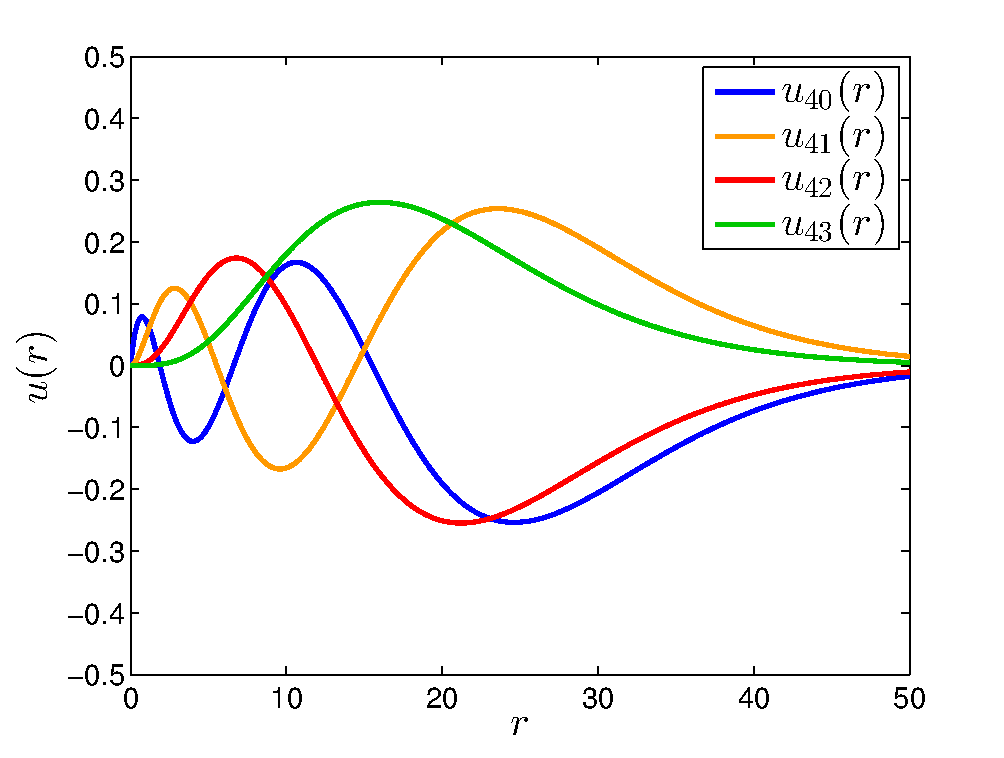
\includegraphics[width=0.325\textwidth]{Z1}\label{fig:Z1}}
\subfloat[][$Z=2$]{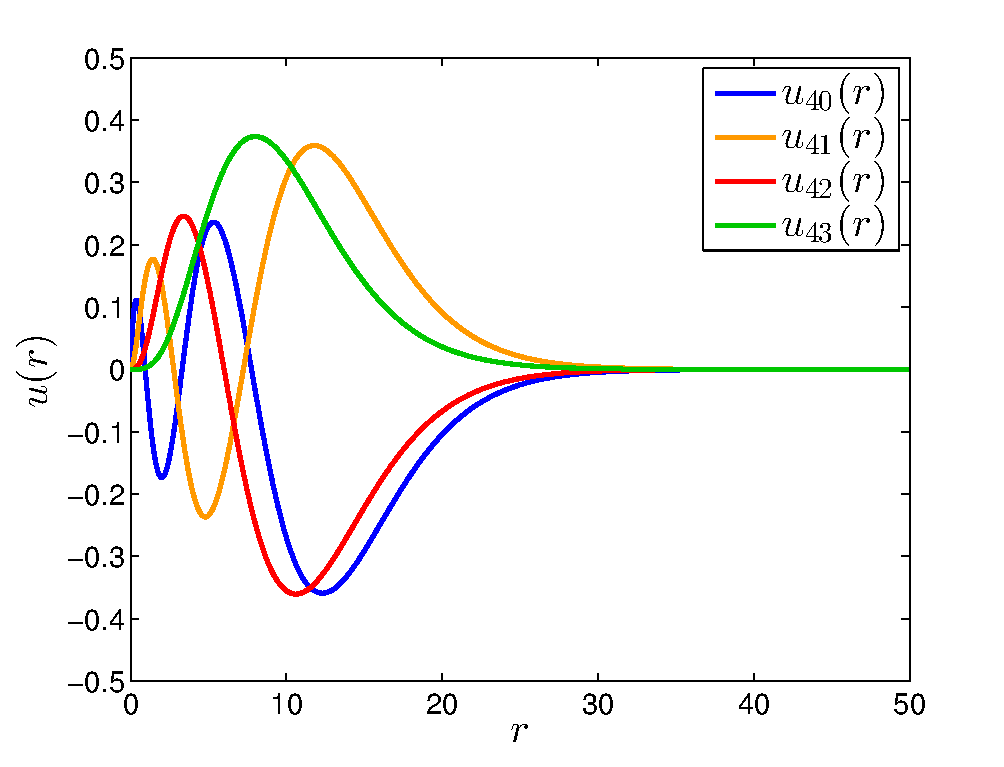
\includegraphics[width=0.325\textwidth]{Z2}\label{fig:Z2}}
\subfloat[][$Z=3$]{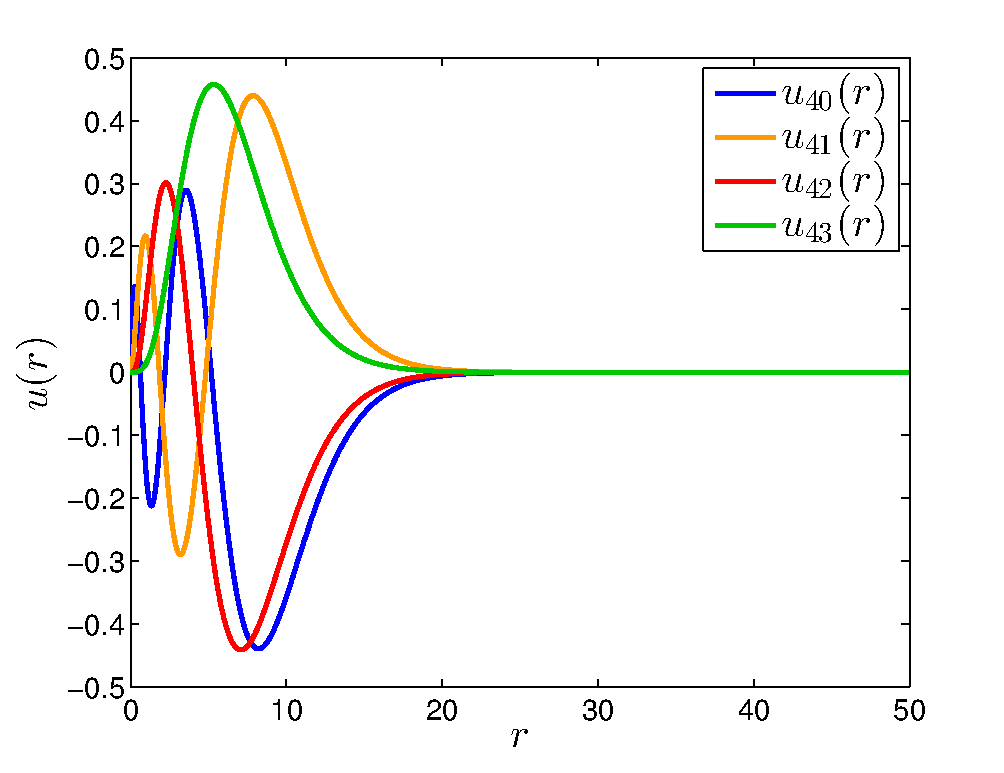
\includegraphics[width=0.325\textwidth]{Z3}\label{fig:Z3}}
\caption{Plots of exact solutions for a few hydrogen-like wave functions with
principal quantum number $n=4$. (a) wave functions of $Z=1$; (b) wave functions of $Z=2$;
(c) wave functions of $Z=3$. The plots demonstrate the smaller $r$ goes,
the stronger is the oscillation of the function $u(r)$. And the wave functions
are attracted more closely to the nucleus with increasing nuclear charge $Z$.}
\label{fig:hydrlike}
\end{figure}

Our choice is to use a logarithmic grid\footnote{The logarithmic grid is not
the unique choice. One can use any adaptive grid as long as it can
properly represent the wave function. But the logarithmic grid uses a change of
variable technique and it is very elegant.} \cite{ES},
$ 0 < r_0 < r_1 < \cdots < r_{n-1} < \infty $, where
\begin{equation} \label{eq:x2r}
r_i = \frac{1}{Z} e^{x_i} \quad\text{or equivalently}\quad \rho_i=e^{x_i}
\end{equation}
\begin{center}
\setlength{\unitlength}{5pt}
\begin{picture}(53.6518,0)
\put(0,0){\line(1,0){53.6518}}
\put(0,0){\line(0,1){1}}
\put(0.2216,0){\line(0,1){1}}
\put(0.4923,0){\line(0,1){1}}
\put(0.8229,0){\line(0,1){1}}
\put(1.2268,0){\line(0,1){1}}
\put(1.7200,0){\line(0,1){1}}
\put(2.3224,0){\line(0,1){1}}
\put(3.0583,0){\line(0,1){1}}
\put(3.9570,0){\line(0,1){1}}
\put(5.0547,0){\line(0,1){1}}
\put(6.3954,0){\line(0,1){1}}
\put(8.0330,0){\line(0,1){1}}
\put(10.0332,0){\line(0,1){1}}
\put(12.4762,0){\line(0,1){1}}
\put(15.4601,0){\line(0,1){1}}
\put(19.1046,0){\line(0,1){1}}
\put(23.5561,0){\line(0,1){1}}
\put(28.9931,0){\line(0,1){1}}
\put(35.6339,0){\line(0,1){1}}
\put(43.7449,0){\line(0,1){1}}
\put(53.6518,0){\line(0,1){1}}
\put(-0.5,-2){$r_0$}
\put(53.1518,-2){$r_{n-1}$}
\end{picture}
\end{center}
and $x$ is a uniformly distributed grid
\begin{equation} \label{eq:xDis}
x_i = x_0 + i \Delta x
\end{equation}
\begin{center}
\setlength{\unitlength}{5pt}
\begin{picture}(53.6520,0)
\put(0,0){\line(1,0){53.6520}}
\put(0,0){\line(0,1){1}}
\put(2.6826,0){\line(0,1){1}}
\put(5.3652,0){\line(0,1){1}}
\put(8.0478,0){\line(0,1){1}}
\put(10.7304,0){\line(0,1){1}}
\put(13.4130,0){\line(0,1){1}}
\put(16.0956,0){\line(0,1){1}}
\put(18.7782,0){\line(0,1){1}}
\put(21.4608,0){\line(0,1){1}}
\put(24.1434,0){\line(0,1){1}}
\put(26.8260,0){\line(0,1){1}}
\put(29.5086,0){\line(0,1){1}}
\put(32.1912,0){\line(0,1){1}}
\put(34.8738,0){\line(0,1){1}}
\put(37.5564,0){\line(0,1){1}}
\put(40.2390,0){\line(0,1){1}}
\put(42.9216,0){\line(0,1){1}}
\put(45.6042,0){\line(0,1){1}}
\put(48.2868,0){\line(0,1){1}}
\put(50.9694,0){\line(0,1){1}}
\put(53.6520,0){\line(0,1){1}}
\put(-0.5,-2){$x_0$}
\put(53.1520,-2){$x_{n-1}$}
\end{picture}
\end{center}

The advantage of this logarithmic grid will be clear in a short while.
First, we introduce a rescaled quantity\footnote{Don't be confused
with the rescalings. As a remark, the relation among $R$, $u$ and $\tilde{u}$
is the following: $R(r) \equiv u(r)/r \equiv \tilde{u}(r)/\sqrt{r}$.}
$\tilde{u} \equiv u/\sqrt{r}$. Recall our analytical solutions in Table~\ref{table:unl},
now instead of $u_{nl}(r)$, we give the relations between $\tilde{u}_{nl}$ and $x$ in
Table~\ref{table:unlt}.

\begin{table}[h!]
\caption{The first few rescaled radial wave functions
$\tilde{u}_{nl}(x)$ for hydrogen-like atoms with atomic number $Z$. The
coordinates $x$ are the logarithmic transformations from the radial coordinate $r$.}
\label{table:unlt}
\begin{equation*}
\renewcommand\arraystretch{1.8}
\begin{array}{|>{\displaystyle}r >{\displaystyle}r >{\displaystyle}l >{\displaystyle}l >{\displaystyle}l|}
  \hline
  \tilde{u}_{10} = & 2                           & Ze^{x/2}  &                                                                    & \exp{(-e^{x})}   \\[0.5em] \hline
  \tilde{u}_{20} = & \frac{1}{\sqrt{2}}          & Ze^{x/2}  & \Big(1-\frac{1}{2}e^{x}\Big)                                       & \exp{(-e^{x}/2)} \\
  \tilde{u}_{21} = & \frac{1}{\sqrt{24}}         & Ze^{3x/2} &                                                                    & \exp{(-e^{x}/2)} \\[0.5em] \hline
  \tilde{u}_{30} = & \frac{2}{\sqrt{27}}         & Ze^{x/2}  & \Big(1-\frac{2}{3}e^{x}+\frac{2}{27}e^{2x}\Big)                    & \exp{(-e^{x}/3)} \\
  \tilde{u}_{31} = & \frac{8}{27\sqrt{6}}        & Ze^{3x/2} & \Big(1-\frac{1}{6}e^{x}\Big)                                       & \exp{(-e^{x}/3)} \\
  \tilde{u}_{32} = & \frac{4}{81\sqrt{30}}       & Ze^{5x/2} &                                                                    & \exp{(-e^{x}/3)} \\[0.5em] \hline
  \tilde{u}_{40} = & \frac{1}{4}                 & Ze^{x/2}  & \Big(1-\frac{3}{4}e^{x}+\frac{1}{8}e^{2x}-\frac{1}{192}e^{3x}\Big) & \exp{(-e^{x}/4)} \\
  \tilde{u}_{41} = & \frac{\sqrt{5}}{16\sqrt{3}} & Ze^{3x/2} & \Big(1-\frac{1}{4}e^{x}+\frac{1}{80}e^{2x}\Big)                    & \exp{(-e^{x}/4)} \\
  \tilde{u}_{42} = & \frac{1}{64\sqrt{5}}        & Ze^{5x/2} & \Big(1-\frac{1}{12}e^{x}\Big)                                      & \exp{(-e^{x}/4)} \\
  \tilde{u}_{43} = & \frac{1}{768\sqrt{35}}      & Ze^{7x/2} &                                                                    & \exp{(-e^{x}/4)} \\[0.5em]
  \hline
\end{array}
\end{equation*}
\end{table}

If we compare Table~\ref{table:unl} and Table~\ref{table:unlt} carefully, we can
find that in the previous formulas, the radial coordinates $r$ are always scaled by a factor
of $Z$, so are the plots in Fig.~\ref{fig:hydrlike}. But with the transformed
coordinate $x$, we no longer have this horizontal scaling and this helps us better work
with heavy nuclei. Meanwhile, the transformed coordinate $x$ ``magnifies'' the
inner region while shrinks the outer. As shown in Fig.~\ref{fig:hydrliket},
we plot the rescaled wave functions with (again) principal quantum number $n=4$
for the three hydrogen-like atoms. In contrast to Fig.~\ref{fig:hydrlike},
the three plots are identical except for a vertical scaling factor $Z$.
The inner regions are magnified clearly and the less important outer regions are reduced.
\begin{figure}[h!]
\centering
\subfloat[][$Z=1$]{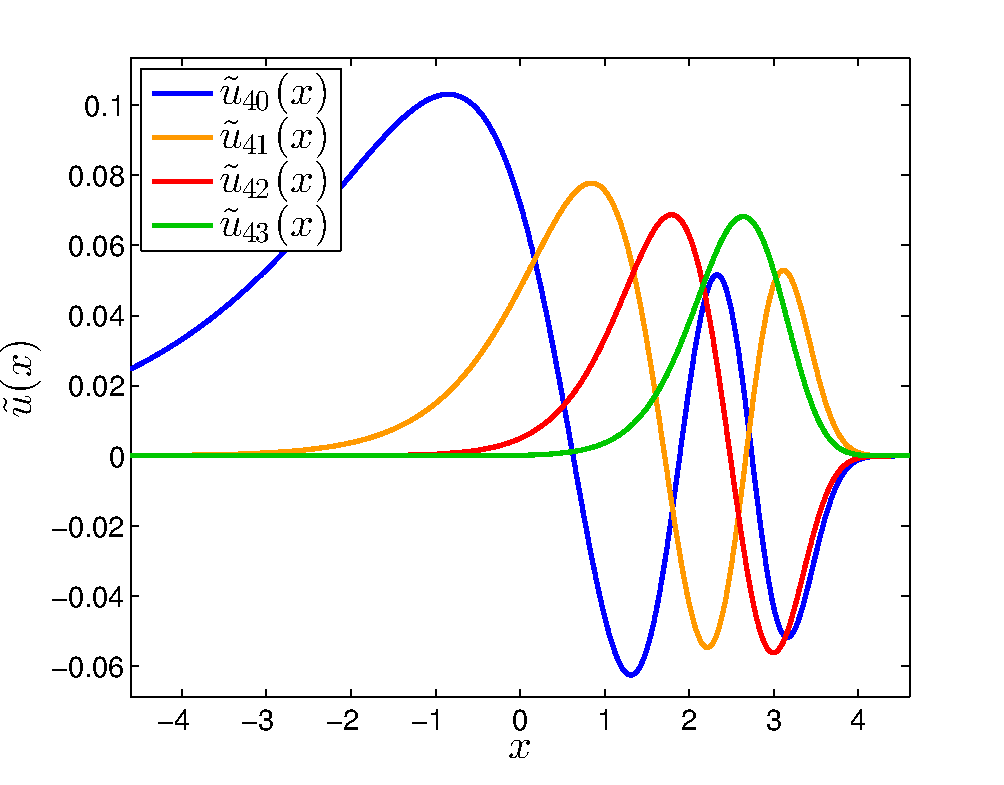
\includegraphics[width=0.325\textwidth]{Z1t}\label{fig:Z1t}}
\subfloat[][$Z=2$]{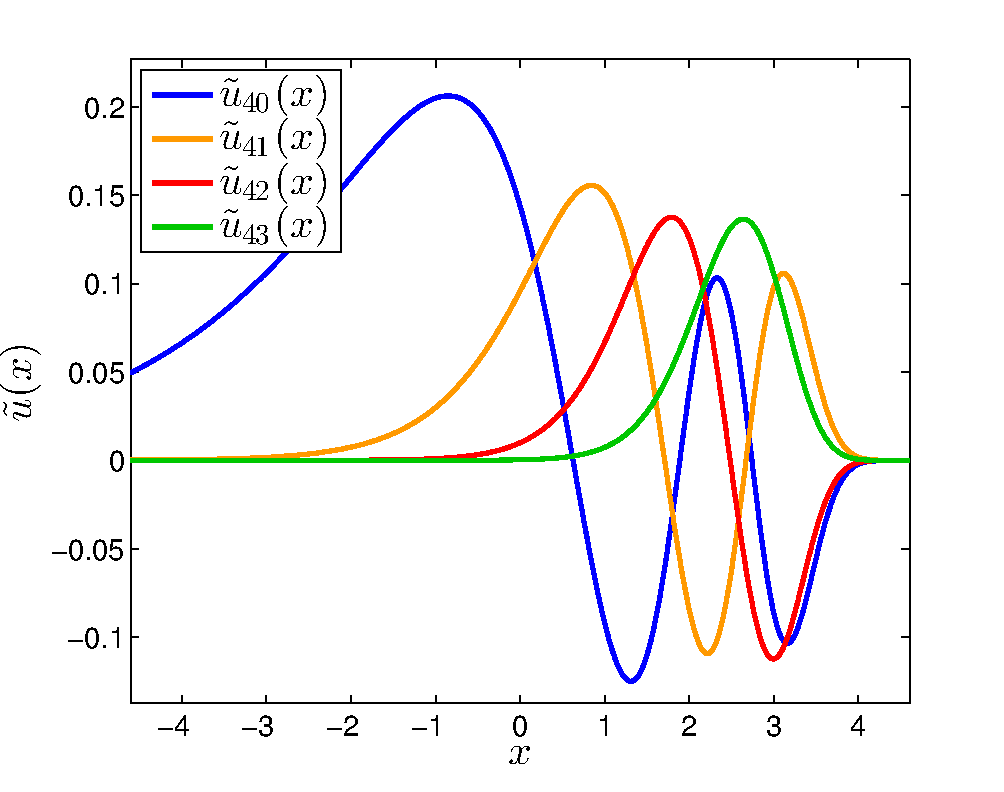
\includegraphics[width=0.325\textwidth]{Z2t}\label{fig:Z2t}}
\subfloat[][$Z=3$]{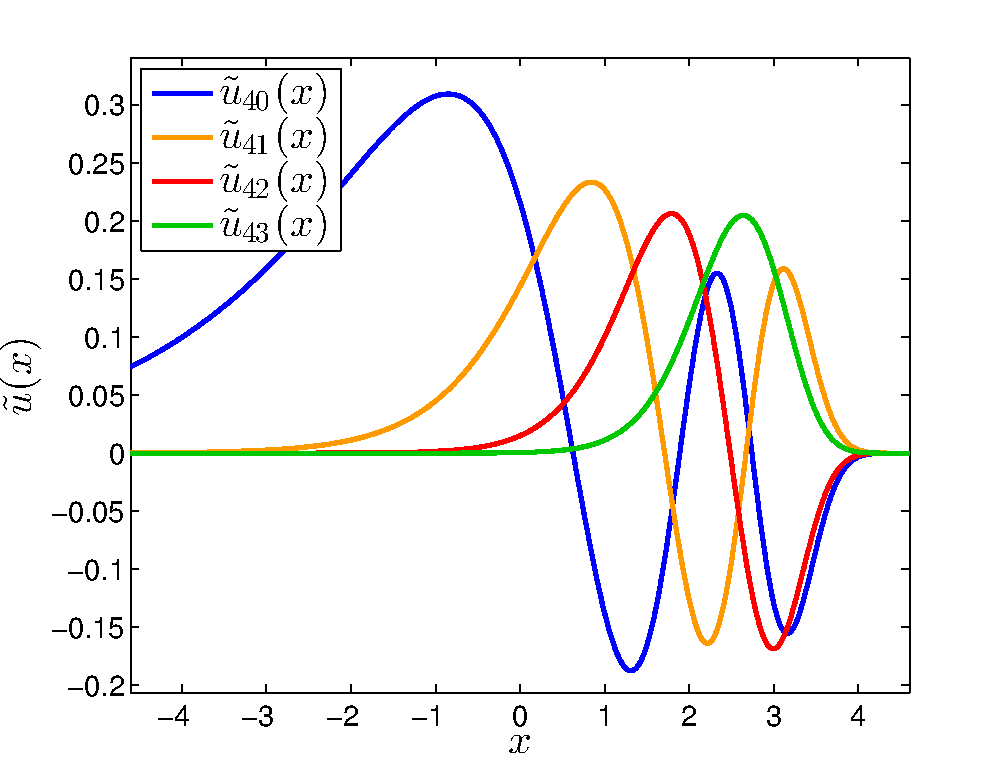
\includegraphics[width=0.325\textwidth]{Z3t}\label{fig:Z3t}}
\caption{The rescaled wave functions with principal quantum number $n=4$
for three hydrogen-like atoms on the transformed grid $x$. (a) wave functions of $Z=1$;
(b) wave functions of $Z=2$; (c) wave functions of $Z=3$. The three plots are
identical except for a vertical scaling factor $Z$. The inner regions
are magnified clearly and the less important outer regions are reduced.}
\label{fig:hydrliket}
\end{figure}

The original problem $u$ on the radial coordinate $r$ can be easily transformed to the
rescaled problem $\tilde{u}$ on the transformed coordinate $x$ by the change of variable
technique. The idea is to replace the second derivative $d^2u/dr^2$ in Eqn.~(\ref{eq:oneElec})
in terms of $d^2\tilde{u}/dx^2$:
\begin{equation} \label{eq:dudx}
\frac{d^2u}{dr^2} = -\frac{1}{4}r^{-3/2} \tilde{u} + r^{-3/2} \frac{d^2 \tilde{u}}{dx^2}
\end{equation}
%
Substituting Eqn.~(\ref{eq:dudx}) into Eqn.~(\ref{eq:oneElec}), we obtain
\begin{equation} \label{eq:oneElecTrans}
-\frac{1}{2} \frac{d^2\tilde{u}}{dx^2} + \left[ r^2 V(r) + \frac{1}{2} \Big(l+\frac{1}{2}\Big)^2 \right] \tilde{u} = r^2 E \tilde{u}
\end{equation}
This is our transformed problem. Now, instead of solving
Eqn.~(\ref{eq:oneElec}) directly, we solve this
transformed equation in (\ref{eq:oneElecTrans}). This logarithmic
transformation is a key to obtaining accurate numerical solutions.

\section{Numerov's method}
The next immediate question is: how to discretize the second derivative in
Eqn.~(\ref{eq:oneElecTrans}) so that we can implement numerical integrations
in our computer program. Perhaps the simplest way is to write this second
derivative in the finite-difference form:
\begin{equation} \label{eq:FD}
\frac{d^2\tilde{u}}{dx^2} \approx \frac{\tilde{u}_{i+1} - 2\tilde{u}_i + \tilde{u}_{i-1}}{\Delta x^2}
\end{equation}
%
This discretization is perfectly valid and we can integrate
Eqn.~(\ref{eq:oneElecTrans}) numerically with 2nd order accuracy.
Nevertheless, there exists a very smart trick which allows us to obtain a 4th
order accurate solution with almost the same amount of computational effort.
This trick is called Numerov's method.

If we take a close look at Eqn.~({\ref{eq:FD}}), we get higher order terms:
\begin{equation} \label{eq:FDhigher}
\frac{d^2\tilde{u}}{dx^2} = \frac{\tilde{u}_{i+1} - 2\tilde{u}_i + \tilde{u}_{i-1}}{\Delta x^2} - \frac{1}{12}\tilde{u}_i^{(4)}\Delta x^2 + \mathcal{O}(\Delta x^4)
\end{equation}
%
But the fourth derivative $\tilde{u}_i^{(4)}$ can be also written in the
finite-difference form:
\begin{equation} \label{eq:FDhigherFD}
\frac{d^2\tilde{u}}{dx^2} = \frac{\tilde{u}_{i+1} - 2\tilde{u}_i + \tilde{u}_{i-1}}{\Delta x^2} - \frac{1}{12}\frac{\tilde{u}_{i+1}^{''} - 2\tilde{u}_i^{''} + \tilde{u}_{i-1}^{''}}{\Delta x^2}\Delta x^2 + \mathcal{O}(\Delta x^4)
\end{equation}
%
Here comes the smart trick, instead of treating the second derivative $\tilde{u}_i^{''}$ in
Eqn.~(\ref{eq:FDhigherFD}) numerically, we can simply replace the $\tilde{u}_i^{''}$
by the relation from the original ODE in (\ref{eq:oneElecTrans}):
\begin{equation} \label{eq:NmvTrick}
\tilde{u}_i^{''} = -2 k_i^2 \tilde{u_i}
\end{equation}
where,
\begin{equation} \label{eq:kk}
k_i^2 \equiv r_i^2 E - r_i^2 V(r_i) - \frac{1}{2} \Big(l+\frac{1}{2}\Big)^2
\end{equation}
%
What remains are simply substitutions. We substitute Eqn.~(\ref{eq:NmvTrick}) into
Eqn.~(\ref{eq:FDhigherFD}) and then substitute Eqn.~(\ref{eq:FDhigherFD}) into
Eqn.~(\ref{eq:oneElecTrans}), we obtain the following relation:
\begin{equation} \label{eq:Numerov}
\boxed{\tilde{u}_{i\pm1} = \frac{(2-\frac{5\Delta x^2}{3}k_i^2)\tilde{u}_i - (1+\frac{\Delta x^2}{6}k_{i\mp1}^2)\tilde{u}_{i\mp1}}{1+\frac{\Delta x^2}{6}k_{i\pm1}^2}}
\end{equation}
%
Eqn.~(\ref{eq:Numerov}) is a simple 3-point recursion: with the knowledge of
$\tilde{u}_{i-1}$ and $\tilde{u}_i$, we can compute $\tilde{u}_{i+1}$ easily
(or from the other direction: to compute $\tilde{u}_{i-1}$ from $\tilde{u}_i$
and $\tilde{u}_{i+1}$).
We are now facing two questions:
\begin{enumerate}
  \item How do we choose the ``starting points'', say, $\tilde{u}_0$
        and $\tilde{u}_1$?
  \item The parameter $k_i^2$ has a dependence on the energy $E$, which is so far
        unknown to us. How do we determine this energy?
\end{enumerate}
Keep those two questions in mind and we will discuss them in detail in the
following section.

\section{The two-sided shooting and matching}
First of all, let's define our grid on which we solve our numerical problem:
\begin{equation} \label{eq:grid}
\left\{ r_{\text{min}} = \frac{0.0001}{Z};\quad r_{\text{max}} = 50.0;\quad \Delta x = 0.002; \right\}
\end{equation}
The minimum of the radial grid $r_{\text{min}}$ depends on the atomic number $Z$,
because the higher the nuclear charge, the closer the electron wave function
will be attracted to the origin. We cannot take $r_{\text{min}}=0$
as $x_{\text{min}} = \ln{(Zr_{\text{min}})}$ will be $-\infty$. The maximum of the radial
grid is a constant $r_{\text{max}} = 50.0$. This consideration is from the fact that the size of
each atom will be roughly the same after self-consistent calculations.\footnote{The
self-consistent calculation will be discussed in a later chapter.
By saying the size of an atom, we mean the distribution range that is covered
by the significant part of the electron wave functions.} Please notice that
we define $\Delta x$ instead of $\Delta r$, because the grid $x_i$ is uniformly
spaced whereas the spacing $\Delta r$ is not a constant.\footnote{As a reference,
number of grid points $\#$: $Z=1\,\rightarrow\,\#=6563$; $Z=10\,\rightarrow\,\#=7713$;
$Z=100\,\rightarrow\,\#=8865$.}

Let's start with the first question we had in our last section: the
initialization of the wave functions. We initialize our wave functions
according to their asymptotes (referring to the boundary conditions
in Eqn.~(\ref{eq:oneElec})):
\begin{alignat}{3} \label{eq:asym}
\tilde{u}(r) & \propto r^{l+1}/\sqrt{r}          && \quad\text{as}\quad r\rightarrow0 \\
\tilde{u}(r) & \propto e^{-\beta r}/\sqrt{r} && \quad\text{as}\quad r\rightarrow\infty
\end{alignat}
%
where $\beta = \sqrt{-2E}$. We perform the numerical integrations from both the forward and the backward
directions.\footnote{One could also implement a one-sided only integration.
However, because of the numerical instability, the solution will diverge out
quickly. A two-sided integration is perhaps the best approach to minimize
the effect of numerical instability.} The corresponding initializations
are summarized in Table~\ref{table:init}.
One might worry about the sign of the energy
$E$ as a positive energy will make the square root imaginary. But we will not
work with positive energies as we are interested only in the bounded states
whose energies are always below zero. A positive energy will result in a scattering
state which is not of our concern here.
%
\begin{table}[h!]
\caption{Wave function initializations for the forward and the backward
directions.}
\label{table:init}
\begin{center}
\begin{tabular}{|c|c|}
  \hline
  & Initialization \\ \hline
  Forward &
  $\begin{aligned}
  \smash[b]{\vphantom{\Big|}}
  \tilde{u}_0 & = r_0^{l+1} / \sqrt{r_0} \\
  \tilde{u}_1 & = r_1^{l+1} / \sqrt{r_1}
  \smash[t]{\vphantom{\Big|}}
  \end{aligned}$ \\ \hline
  Backward &
  $\begin{aligned}
  \smash[b]{\vphantom{\Big|}}
  \tilde{u}_{n-1} & = e^{-\beta r_{n-1}} / \sqrt{r_{n-1}} \\
  \tilde{u}_{n-2} & = e^{-\beta r_{n-2}} / \sqrt{r_{n-2}}
  \smash[t]{\vphantom{\Big|}}
  \end{aligned}$ \\
  \hline
\end{tabular}
\end{center}
\end{table}

Be careful there is a pitfall in the backward initialization. Let's say we take
$r_{n-1} = 50$ and $E = -300$. The term $e^{-\beta r_{n-1}}$ will have
a value approximately $1.26\times10^{-532}$, which is such a small number that
cannot be represented by a double precision floating point number. As a result,
this initialization will return us $0$.
But if $\tilde{u}_{n-1}$ and $\tilde{u}_{n-2}$ are zeros, the resulting
$\tilde{u}_{n-3}$, $\tilde{u}_{n-4}$, $\ldots$ from the integration
in Eqn.~(\ref{eq:Numerov}) will all become zeros.
And of course this is not what we wanted. To overcome this problem, we should
keep doing the initialization for $\tilde{u}_{n-3}$, $\tilde{u}_{n-4}$, $\ldots$
until we meet the first $\tilde{u}_i$ which is nonzero. And this $\tilde{u}_i$
and the next $\tilde{u}_{i-1}$ will be our starting points for the backward integrations.
Actually the same argument applies to the forward initialization. If $r_0$
goes extremely small, $\tilde{u}_0$ will also have an arithmetic underflow
problem. However, unlike the exponential term in the backward initialization,
this value will not drop to zero that quickly. In our practical problems, we do
not need to worry about the underflow problems in the forward direction and can simply
assign the initial values to $\tilde{u}_0$ and $\tilde{u}_1$.

There is one important hidden message in Eqn.~(\ref{eq:Numerov}):
If any two adjacent points (not necessarily the end ones) are given,
the entire wave function can be reconstructed. This is the underlying
principle of how one should match the wave functions from the forward and
backward integrations. Ideally, if $E$ is an eigen-energy, the resulting
wave functions from the forward and backward integrations will be identical
(up to a normalization\footnote{Normalization of wave functions will be
discussed in the later section.} factor). On the other hand, if $E$ is not an
eigen-energy, the wave functions will not match. To check whether two wave functions
matched or not, we do not compare the entire wave functions (they
will never match due to numerical instability). What we should match instead
are two adjacent points on the two wave functions.
As we mentioned before, if the solutions agree in two points, in principle
they will agree everywhere. But which two points do we compare?
Apparently, those two points should not be too close to the boundaries. Because of
numerical instability, the wave functions will diverge out quickly if integrating
into classically forbidden regions. A good choice of these two points could be around
the classical turning point. A classical turning point is the position where
the energy of the electron is equal to the potential\footnote{The true classical turning
point should be at $E=V_{\text{eff}}(r)$ where $V_{\text{eff}}(r)=V(r)+\frac{l(l+1)}{2r^2}$.
But it is better to only use $V(r)$ here since $V_{\text{eff}}(r)$ will introduce an additional
root near the origin.} $E=V(r)$. Beyond the classical turning point,
the electron reaches the classically forbidden region. And inside this region,
the electron wave function will decay exponentially and no further node\footnote{A node
is a point along the wave function where the wave function goes through zero.
See Fig.~\ref{fig:hydrlike} and Fig.~\ref{fig:hydrliket} for example.} will
be created. Our matching points $r_{\text{M1}}$ and $r_{\text{M2}}$ (they are adjacent)
are taken such that $E \ge V(r_{\text{M1}})$ and $E<V(r_{\text{M2}})$ (see Fig.~\ref{fig:r1r2}).
A so called matched wave function satisfies the following criterion,
\begin{equation} \label{eq:crit}
\big|\tilde{u}_{\text{F}1} \tilde{u}_{\text{B}2} - \tilde{u}_{\text{F}2} \tilde{u}_{\text{B}1}\big| < \varepsilon
\end{equation}
where $\varepsilon$ is a small tolerance, say, $\varepsilon=10^{-8}$.
The subscripts ``F'' and ``B'' denote whether the wave function comes
form the forward integration or from the other direction. One might ask
why don't we simply compare the two points such that
$|\tilde{u}_{\text{F}1} - \tilde{u}_{\text{B}1}| < \varepsilon$
and $|\tilde{u}_{\text{F}2} - \tilde{u}_{\text{B}2}| < \varepsilon$.
But we should understand that the two wave functions from the forward and backward
directions need to match only up to a normalization factor.
The initialization in Table~\ref{table:init} does not guarantee that
the wave functions from the two directions will have the same scaling factor.
\begin{figure}[h!]
\centering
  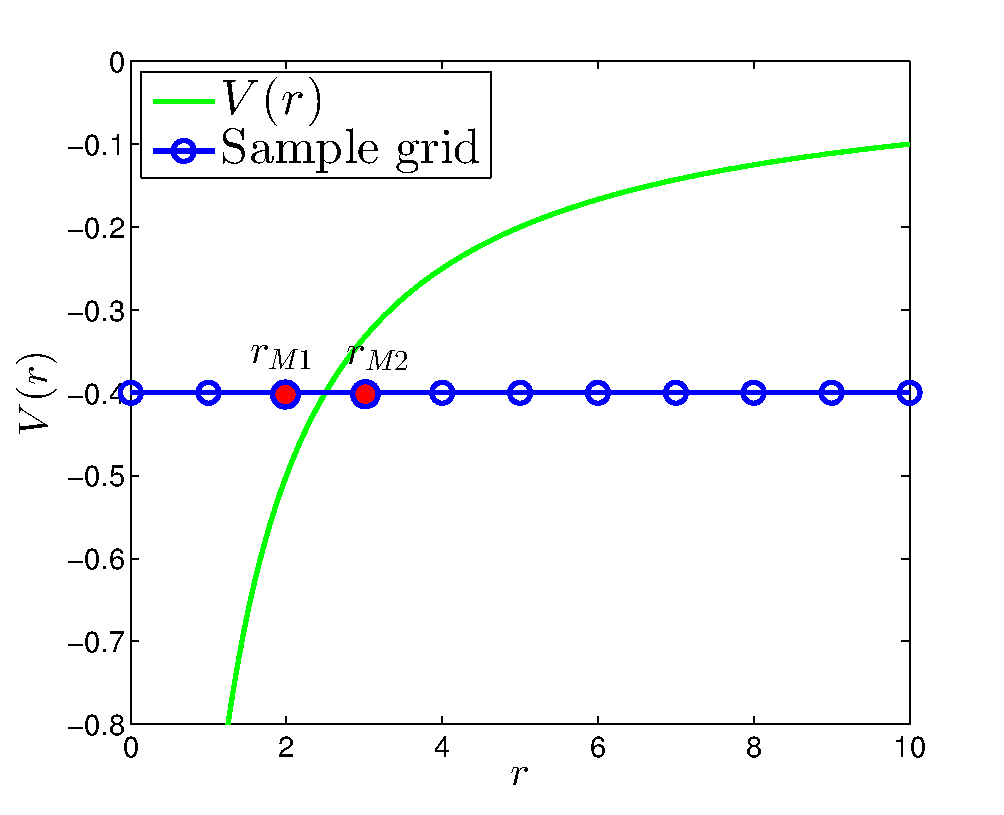
\includegraphics[width=0.45\textwidth]{r1r2}
  \caption{Two matching points when $E=-0.4$ with potential $V(r)=-1/r$ on a sample grid.}
  \label{fig:r1r2}
\end{figure}

As an important note, instead of comparing the two points, many people would
like to compare the first derivatives of the two wave functions at a matching position.
That is also very intuitive as a matched wave function should be ``smooth''. However,
comparing the first derivatives will introduce additional numerical error unless the
derivative is calculated with a formula consistent with the Numerov's integration.
The comparison of two adjacent points does that automatically, which will give us
a 4th order accuracy that is consistent with the Numerov's method.

So, everything is ready. What remains is to determine the electron energy $E$.
Believe it or not, the determination of $E$ is a trial-and-error approach.
As demonstrated in Fig.~\ref{fig:match}, we first make a guess to the energy
$E=-0.6$. Then we perform the integration (the so called shooting) and find
out the wave functions at the matching point do not match and the guessed
energy was too low. Next we increase our energy $E=-0.4$ and realize the
energy is too high this time. Finally, by trial-and-error, we lock on the
eigen-energy which in this case should be $E=-0.5$. This trial-and-error strategy
is actually the spirit of the shooting and matching method.

\begin{figure}[h!]
\centering
\subfloat[][$E=-0.6$]{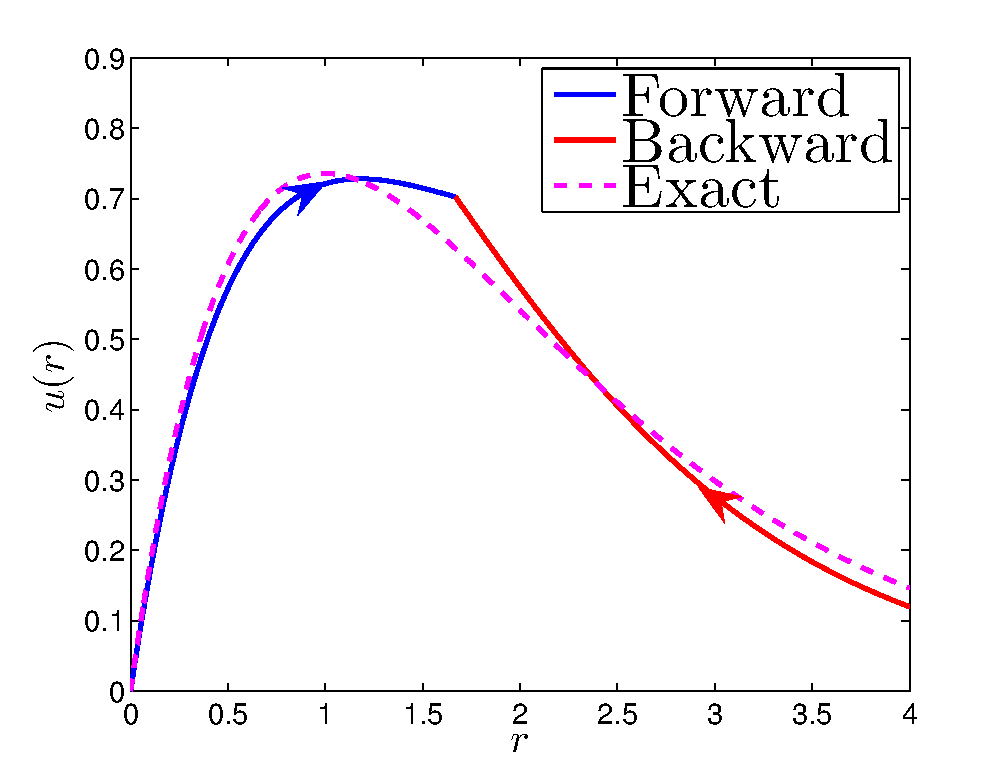
\includegraphics[width=0.325\textwidth]{E06}\label{fig:E06}}
\subfloat[][$E=-0.4$]{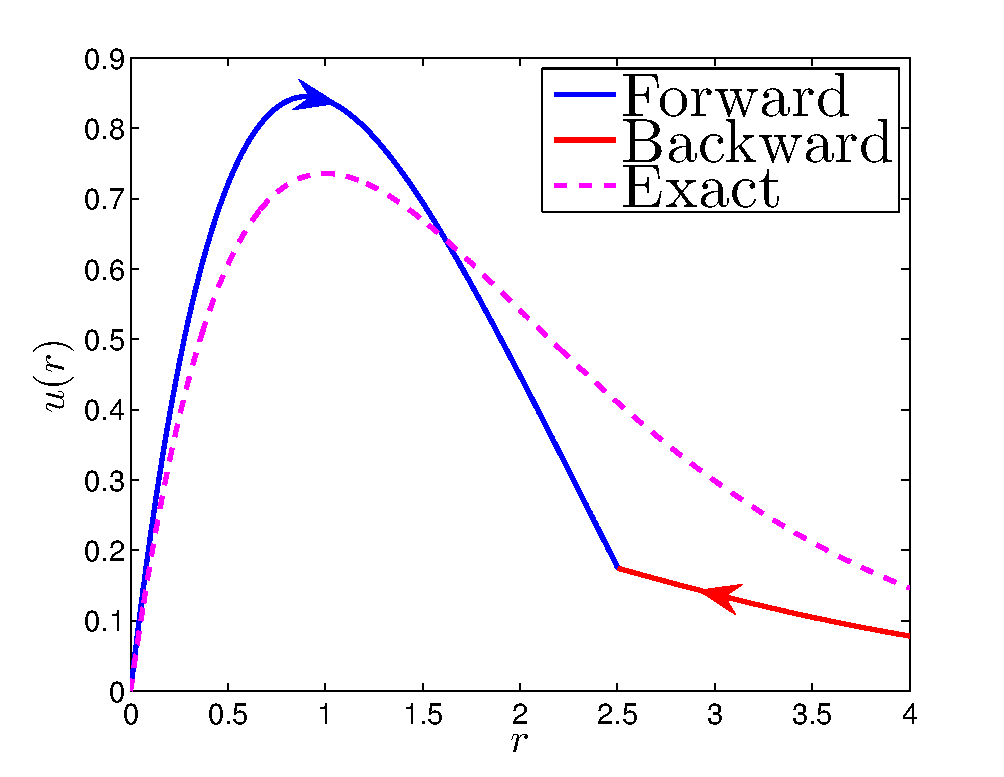
\includegraphics[width=0.325\textwidth]{E04}\label{fig:E04}}
\subfloat[][$E=-0.5$]{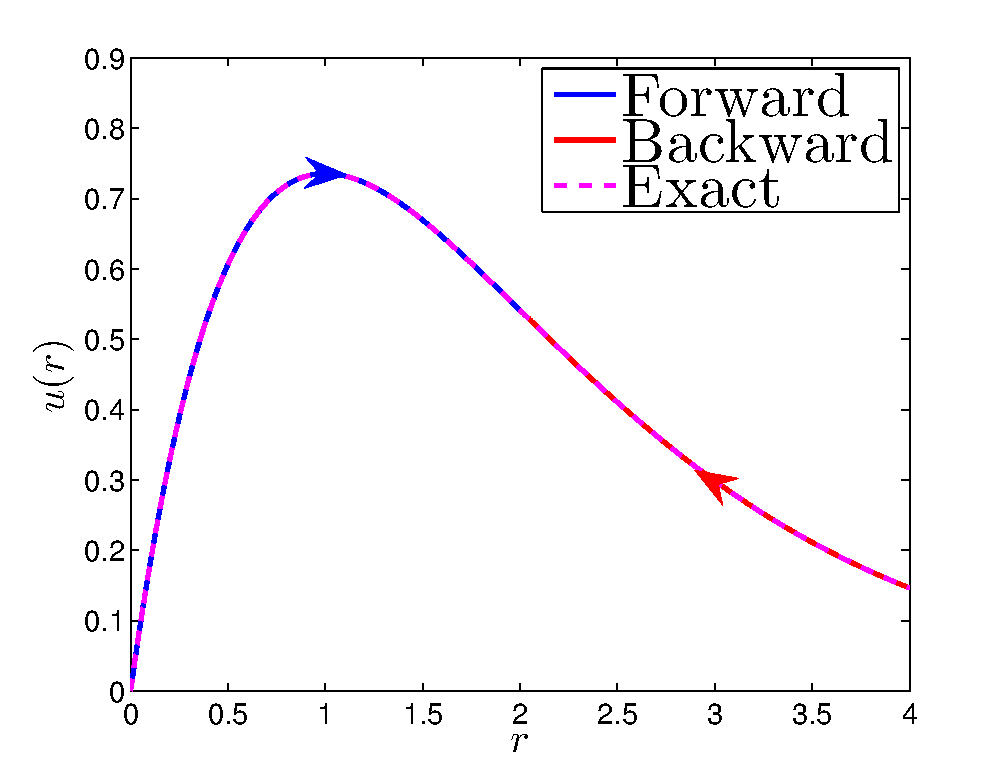
\includegraphics[width=0.325\textwidth]{E05}\label{fig:E05}}
\caption{Forward integration and backward integration matching for the wave
function $u_{10}$ of a hydrogen atom ($Z=1$). It is really a trial-and-error
strategy to determine the eigen-energy.}
\label{fig:match}
\end{figure}

\section{The bisection method}
Suppose we have our program codes ready, our next job is to modify the parameter
$E$ and run the program over and over to find out the possible eigen-energies and
the corresponding eigen-functions. This is a rather tedious job. But an experienced
programmer (like us) will soon notice that we could let the machine do this trial-and-error
process automatically.

This automation procedural is called the bisection method. The idea is to start
from two initial guesses $E_{\text{low}}$ and $E_{\text{up}}$, and locate the
solution\footnote{It is very likely that more than one eigen-states are in
between $E_{\text{low}}$ and $E_{\text{up}}$. But the algorithm for finding all of them will
be more complicated and one has to be more careful for that situation. For
simplicity, here we only provide an algorithm for locating one eigen-state.}
in between. We provide the bisection algorithm for identifying the
eigen-states in Algorithm~\ref{alg:bisect}.

\begin{algorithm}[h!]
\caption{Bisection method}\label{alg:bisect}
\begin{algorithmic}[1]
\Function{Bisection}{$E_{\text{low}}$, $E_{\text{up}}$}
\State $eigen_{\text{low}} \gets$ \Call{Shoot}{$E_{\text{low}}$}
\State $eigen_{\text{up}} \gets$ \Call{Shoot}{$E_{\text{up}}$}
\State $match_{\text{low}} \gets eigen_{\text{low}}.match$
\State $match_{\text{up}} \gets eigen_{\text{up}}.match$
\State $node_{\text{low}} \gets eigen_{\text{low}}.node$
\State $node_{\text{up}} \gets eigen_{\text{up}}.node$
\If {$node_{\text{up}}-node_{\text{low}} = 1$
{\bf and} $match_{\text{up}}*match_{\text{low}} < 0$}
\Loop
\State $E \gets (E_{\text{low}}+E_{\text{up}})/2$
\State $eigen \gets$ \Call{Shoot}{$E$}
\State $match \gets eigen.match$
\If {$|match| < \varepsilon$} \Comment {Eigen-state found}
\State \Return $eigen$
\Else
\If {$match*match_{\text{low}} > 0$}
\State $E_{\text{low}} \gets E$
\State $match_{\text{low}} \gets match$
\ElsIf {$match*match_{\text{up}} > 0$}
\State $E_{\text{up}} \gets E$
\State $match_{\text{up}} \gets match$
\Else
\State \Return false
\EndIf
\EndIf
\EndLoop
\Else
\State \Return false
\EndIf
\EndFunction
\end{algorithmic}
\end{algorithm}

The mysterious function \texttt{Shoot}() in Algorithm~\ref{alg:bisect} is
basically the initialization and Numerov integration that we discussed in
previous sections. The function \texttt{Shoot}() takes an argument $E$ and
returns an object which contains all the essential information of the resulting
wave function, including the energy, the normalized wave function, number
of nodes, the matching quality (as defined
in Eqn.~(\ref{eq:crit})), etc. The difference between the number of nodes
from $E_{\text{low}}$ and $E_{\text{up}}$ determines the number of
eigen-states between them. As a remark, there is a close relation among
the number of nodes, the principal quantum number and the orbital angular
momentum quantum number: $n = node + l + 1$.

\section{Normalizing the wave function}
In the previous sections, we mentioned the wave function normalization. By saying
normalizing a wave function, it means to find a factor $A$ such that
\begin{equation} \label{eq:norm}
A \int_0^\infty dr\,|u|^2 = 1
\end{equation}
The re-assignment $u \gets \sqrt{A}u$ normalizes the wave function.

It is now a matter of how to evaluate this integral numerically. First of all,
it would be convenient if we transform our problem onto the uniform grid $x$.
By change of variable $dr = (dr/dx)dx$, Eqn.~(\ref{eq:norm}) becomes
\begin{equation} \label{eq:normt}
A \int_0^\infty dx\,r\,|u|^2 = 1
\end{equation}
%
There are three standard numerical methods to compute the definite integrals.
The first one, which is the simplest, will be exact if the integrand $f(x)$ is
a piecewise constant function. It is called the rectangle rule.
\begin{equation} \label{eq:rect}
\int_{x_0}^{x_{n-1}} dx\,f(x) \approx \Delta x \sum_{i=0}^{n-2}{f(x_i)}
\end{equation}
%
The second one, the trapezoidal rule, will be exact if the integrand
is piecewise linear.
\begin{equation} \label{eq:tpzd}
\int_{x_0}^{x_{n-1}} dx\,f(x) \approx \frac{\Delta x}{2} \sum_{i=0}^{n-2}{\left[f(x_i) + f(x_{i+1})\right]}
\end{equation}
%
The next order is quadratic. The Simpson's rule does an interpolation on each
3-point stencil. It is exact when the integrand is piecewise quadratic.
In order to concatenate every 3-point stencil together,
it requires the total number of the grid points to be odd.
The Simpson's rule is often more accurate than the rectangle and
trapezoidal rules. Here I use $(+2)$ in the summation to denote the index $i$ jumps
in steps of 2.
\begin{equation} \label{eq:simp}
\int_{x_0}^{x_{n-1}} dx\,f(x) \approx \frac{\Delta x}{3} \left[f(x_0) + 4\sum_{i=1(+2)}^{n-2}{f(x_i)} + 2\sum_{i=2(+2)}^{n-3}{f(x_i)} + f(x_{n-1})\right]
\end{equation}
%
To compare those three methods, we calculate the numerical results
for the following sample integration (whose analytical solution can be computed easily):
\begin{equation} \label{eq:sampInt}
\int_{x_0}^{x_{n-1}} dx\,r\,\sin{(x)}
\end{equation}
on a few grids with different spacing:
\begin{equation} \label{eq:sampIntGrid}
\left\{ r_{\text{min}} = 1.0;\quad r_{\text{max}} = 50.0;\quad \Delta x = 10^0,10^{-1},\ldots,10^{-6}; \right\}
\end{equation}
%
We plot the relative error against the grid size $\Delta x$
on a log-log scale for the three methods, rectangle, trapezoidal
and Simpson. The results are shown in Fig.~\ref{fig:rts}.
In the log-log scale plot, the slope of each curve indicates the order
of accuracy of each method. Apparently, the Simpson's rule gives
the highest order among the three methods. There is a ``turning point''
on the Simpson's curve around $\Delta x = 10^{-3}$, since the solution hits
the machine precision. In our shooting method problems, we have a grid
with $\Delta x = 0.002$ and the Simpson's rule is our choice.

\begin{figure}[h!]
\centering
  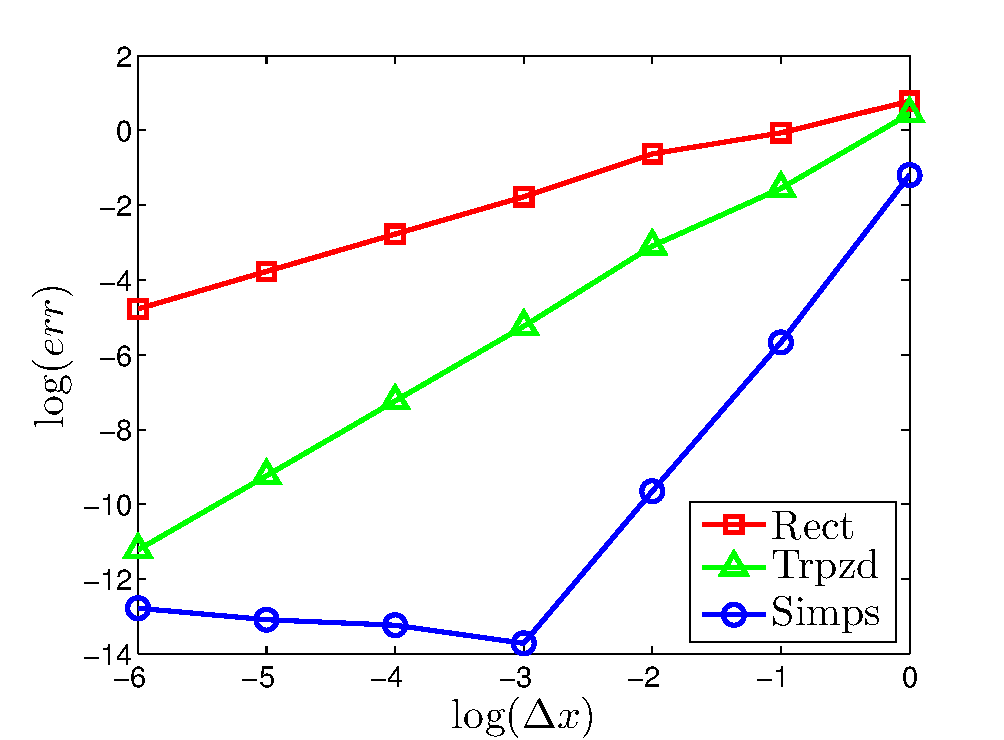
\includegraphics[width=0.5\textwidth]{rts}
  \caption{Numerical integrations for $f(x)=r\sin{(x)}$ using
  rectangle, trapezoidal and Simpson's rules. This figure plots the relative
  error against the grid size $\Delta x$ on a log-log scale. 
  The slope of each curve indicates the order of the accuracy.}
  \label{fig:rts}
\end{figure}

\section{Numerical and exact eigen-energy comparison}
To confirm the correctness of our results and to check the accuracy, we can
compare our numerical solutions with the analytical eigen-energies of hydrogen-like
atoms. The eigen-energies of a hydrogen-like atom is given by (in Hartree)
\begin{equation} \label{eq:eigE}
E_n = -\frac{Z^2}{2n^2}
\end{equation}
%
We selected a few one-electron ions for comparison, namely H ($Z=1$), $\text{C}^{5+}$ ($Z=6$),
$\text{Fe}^{25+}$ ($Z=26$), $\text{Ag}^{46+}$ ($Z=47$) and $\text{U}^{91+}$ ($Z=92$).
Please notice that they are not neutral atoms, but with only one electron inside
(this is what we are able to deal with up to this stage). Table~\ref{table:eigE} lists the numerical
and exact eigen-energies for the selected elements. Energies are given in
units of Hartree (a.u.). The absolute error $e_{\text{abs}} = |E_{\text{num}} - E_{\text{exa}}|$
and the relative error $e_{\text{rel}} = |(E_{\text{num}} - E_{\text{exa}})/E_{\text{exa}}|$
are listed accordingly. The symbols in column 2 are the orbital names. For
instance, $2p$ is an orbital with principal quantum number $n=2$ and orbital angular momentum
quantum number $l=1$. A direct mapping between $l$ and its ``name'' is given below:
\begin{center}
\begin{tabular}{ c | c | c | c | c | c | c }
  \hline
  $l$          & 0 & 1 & 2 & 3 & 4 & 5 \\ \hline
  orbital name & $s$ & $p$ & $d$ & $f$ & $g$ & $h$ \\
  \hline
\end{tabular}
\end{center}

With this nicely tabulated result, we conclude our one-electron system computation
in this section. From the next chapter, we will start to work on with more
complicated, more realistic and of course more exciting cases, the many-electron systems.

\begin{table}[h!]
\caption{The numerical and exact eigen-energies for the selected
one-electron atoms. Energies are given in units of Hartree (a.u.).}
\label{table:eigE}
\begin{center}
\begin{tabular}{ c | c | r | r | r | r }
  \hline
 Elem & Orbital & Numerical & Exact & Abs Error & Rel Error \\ \hline \hline
  H &  $1s$  &  $-0.500000$  &  $-0.500000$  &  0.000000  &  0.000000 \\  \hline
  C &  $1s$  &  $-18.000002$  &  $-18.000000$  &  0.000002  &  0.000000 \\ 
    &  $2s$  &  $-4.499999$  &  $-4.500000$  &  0.000001  &  0.000000 \\ 
    &  $2p$  &  $-4.500001$  &  $-4.500000$  &  0.000001  &  0.000000 \\  \hline
 Fe &  $1s$  &  $-338.000032$  &  $-338.000000$  &  0.000032  &  0.000000 \\ 
    &  $2s$  &  $-84.499984$  &  $-84.500000$  &  0.000016  &  0.000000 \\ 
    &  $2p$  &  $-84.500012$  &  $-84.500000$  &  0.000012  &  0.000000 \\ 
    &  $3s$  &  $-37.555556$  &  $-37.555556$  &  0.000000  &  0.000000 \\ 
    &  $3p$  &  $-37.555556$  &  $-37.555556$  &  0.000000  &  0.000000 \\
    &  $3d$  &  $-37.555555$  &  $-37.555556$  &  0.000001  &  0.000000 \\
    &  $4s$  &  $-21.125000$  &  $-21.125000$  &  0.000000  &  0.000000 \\ \hline
 Ag &  $1s$  &  $-1104.500105$  &  $-1104.500000$  &  0.000105  &  0.000000 \\ 
    &  $2s$  &  $-276.124947$  &  $-276.125000$  &  0.000053  &  0.000000 \\ 
    &  $2p$  &  $-276.125039$  &  $-276.125000$  &  0.000039  &  0.000000 \\ 
    &  $3s$  &  $-122.722225$  &  $-122.722222$  &  0.000003  &  0.000000 \\ 
    &  $3p$  &  $-122.722225$  &  $-122.722222$  &  0.000003  &  0.000000 \\ 
    &  $3d$  &  $-122.722219$  &  $-122.722222$  &  0.000003  &  0.000000 \\ 
    &  $4s$  &  $-69.031250$  &  $-69.031250$  &  0.000000  &  0.000000 \\ 
    &  $4p$  &  $-69.031250$  &  $-69.031250$  &  0.000000  &  0.000000 \\
    &  $4d$  &  $-69.031250$  &  $-69.031250$  &  0.000000  &  0.000000 \\
    &  $5s$  &  $-44.180001$  &  $-44.180000$  &  0.000001  &  0.000000 \\ \hline
  U &  $1s$  &  $-4232.000404$  &  $-4232.000000$  &  0.000404  &  0.000000 \\ 
    &  $2s$  &  $-1057.999798$  &  $-1058.000000$  &  0.000202  &  0.000000 \\ 
    &  $2p$  &  $-1058.000151$  &  $-1058.000000$  &  0.000151  &  0.000000 \\ 
    &  $3s$  &  $-470.222232$  &  $-470.222222$  &  0.000010  &  0.000000 \\ 
    &  $3p$  &  $-470.222232$  &  $-470.222222$  &  0.000010  &  0.000000 \\ 
    &  $3d$  &  $-470.222210$  &  $-470.222222$  &  0.000012  &  0.000000 \\ 
    &  $4s$  &  $-264.500000$  &  $-264.500000$  &  0.000000  &  0.000000 \\ 
    &  $4p$  &  $-264.500000$  &  $-264.500000$  &  0.000000  &  0.000000 \\ 
    &  $4d$  &  $-264.500000$  &  $-264.500000$  &  0.000000  &  0.000000 \\
    &  $4f$  &  $-264.500000$  &  $-264.500000$  &  0.000000  &  0.000000 \\ 
    &  $5s$  &  $-169.280006$  &  $-169.280000$  &  0.000006  &  0.000000 \\ 
    &  $5p$  &  $-169.280006$  &  $-169.280000$  &  0.000006  &  0.000000 \\ 
    &  $5d$  &  $-169.280006$  &  $-169.280000$  &  0.000006  &  0.000000 \\
    &  $5f$  &  $-169.280000$  &  $-169.280000$  &  0.000000  &  0.000000 \\ 
    &  $6s$  &  $-117.555553$  &  $-117.555556$  &  0.000003  &  0.000000 \\ 
    &  $6p$  &  $-117.555553$  &  $-117.555556$  &  0.000003  &  0.000000 \\ 
    &  $7s$  &  $-86.367345$  &  $-86.367347$  &  0.000002  &  0.000000 \\ 
  \hline  
\end{tabular}
\end{center}
\end{table}
